\documentclass[../main/main.tex]{subfiles}

\begin{document}
\espacio

  En este capítulo se muestra en detalle la problemática de la investigación.

  \section{Determinación del problema}

  La CPU ejecuta las tareas que le son asignadas de acuerdo a una secuencia definida mediante criterios de prioridad o tiempos de llegada, estos procesos pueden ser a su vez pausados para resolver tareas con un mayor nivel de criticidad de acuerdo al algoritmo de planificación de colas que la CPU utilice; de esta manera, estas tareas ingresan a una cola de espera, que dependiendo del trabajo de la CPU, pueden tardar un tiempo considerable en ser atendidos, e inclusive desecharse por la excesiva carga de trabajo de la CPU. En las comunicaciones encriptadas, dada la lógica inherente de los procesos de encriptación, los tiempos de ejecución pueden llegar a incrementarse hasta un punto insostenible para un solo procesador, por lo cual los fabricantes, de acuerdo a las limitaciones de tamaño y frecuencia máxima de la CPU, vieron necesario el incremento del número de procesadores a fin de atender los procesos en la cola y evitar desechar tareas por los tiempos excesivos de ejecución.

  Para resolver este problema se plantea la alternativa de procesamiento descentralizado mediante la delegación de trabajos a la GPU; a su vez, se medirá la diferencia de tiempos mediante la comparación del tiempo de ejecución del Algoritmo de Encriptación Avanzada AES Rijndael ejecutado en la CPU versus el tiempo de ejecución del proceso en la GPU haciendo uso del entorno de programación Python, que cabe señalar, cuenta con compatibilidad nativa para la ejecución de tareas en matrices de procesadores CUDA mediante la librería Numba\footnote{\href{http://numba.pydata.org/numba-doc/latest/cuda/index.html}{NumPy+Mamba=Numba: Array-oriented Python Compiler for NumPy}}.

  \section{Límites y alcances} \label{limites_alcances}

  El algoritmo utilizado y modificado para la obtención de resultados en CPU y GPU, cumple con la definición de la Publicación de Estándares de Procesamiento de Información Federal 197\footnote{Federal Information Processing Standards Publications - FIPS 197}. [\cite{report:FIPS_197}]. Dicha publicación fue aprobada por el Instituto Nacional de Estándares y Tecnología\footnote{National Institute of Standards and Technology - NIST} después de la verificación en la Reforma de Administración de Tecnologías de la Información\footnote{Information Technology Management Reform} de 1996.

  El relleno de datos de 128 bits cumple con el Estándar de Criptografía de Llave Pública PKCS \#7 plasmado en el reporte RFC 2315 [\cite{report:RFC_2315}].

  \begin{figure}[H]
    \centering
    \caption{Microprocesador Intel i7-3770}
    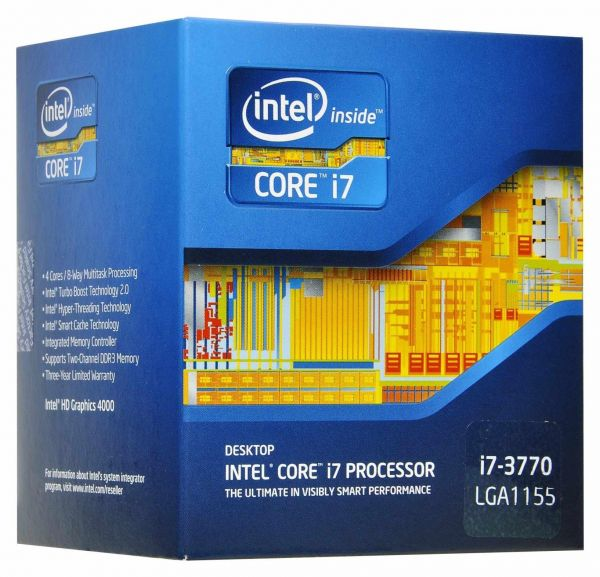
\includegraphics[width=7cm, keepaspectratio]{problema/intel_i7.jpg}
    \caption*{\textbf{Fuente:} \href{https://tinyurl.com/yb3tqpvu}{Intel® Core™ i7-3770 Processor, ark.intel.com}}
  \end{figure}

  En cuanto al hardware, se realiza la comparación de tiempo de ejecución en el microprocesador Intel i7-3770\footnote{\href{https://tinyurl.com/yb3tqpvu}{Intel® Core™ i7-3770 Processor, ark.intel.com}} con respecto a la tarjeta gráfica NVidia GTX 650 Ti\footnote{\href{https://tinyurl.com/ycr3kouv}{NVidia GeForce GTX-650Ti, www.geforce.com}}. Lo que representa una comparativa de trabajo simultáneo de 8 núcleos trabajando a 3.4GHz versus 768 núcleos trabajando a 928MHz para las operaciones pasibles a paralelismo.

  El algoritmo, modificado para esta investigación, fue escrito originalmente por Pablo Caro y es de código abierto, se puede encontrar en la plataforma Github\footnote{\href{https://github.com/pcaro90/Python-AES}{Python-AES, Pablo Caro}}. El código original no cuenta con ninguna ejecución de procesos en paralelo.

  \begin{figure}[H]
    \centering
    \caption{Tarjeta Gráfica NVidia GeForce GTX-650Ti}
    
\includegraphics[width=12cm, keepaspectratio]{problema/gtx_650ti.png}
    \caption*{\textbf{Fuente:} \href{https://tinyurl.com/ycr3kouv}{NVidia GeForce GTX-650Ti, www.geforce.com}}
  \end{figure}

  Se realizaron modificaciones al algoritmo mencionado anteriormente mediante la librería Numba que cuenta con decoradores predefinidos que compilan el código para que pueda ser paralelizado. Esta librería genera kernels compatibles con plataformas CUDA de distintas arquitecturas.

  El sistema operativo utilizado para la investigación es Arch Linux con el Kernel versión 4.18.10.

  El driver de NVidia que se utilizó es de la versión 410.57-2 con el manejador de procesadores CUDA versión 10.0.130-2.

  La versión de Python utilizada fue 3.6.7, con las librerías externas Numba v0.41 y Numpy v1.15.1.
\end{document}